\section{Review of Graph Neural Networks}

In this section, we introduce the concepts related to the graph neural network and breifly survey typical graph neural networks.
We denote a simple graph $\mathcal{G}$ as $\mathcal{G}=(\mathcal{V}, \mathcal{E})$, where $\mathcal{V}$ and $\mathcal{E}$ are the vertex set and the edge set of $\mathcal{G}$, respectively.
Let $n=|\mathcal{V}|$ and $m=|\mathcal{E}|$ as the number of vertices/edges. 
We use $v_i$ $(0 \leq i < n)$ to denote a vertex and $e_{i,j}=(v_i, v_j)$ to denote the edge pointing from $v_i$ to $v_j$.
The adjacency set of $v_i$ is $\mathcal{N}(v_i)=\{v|(v_i, v) \in \mathcal{E}\}$.
We denote a \emph{vector} with a bold lower case letter like $\boldsymbol{x}$ and a \emph{matri}x with a bold upper case letter like $\boldsymbol{X}$.

\subsection{General Structure of Graph Neural Networks}

As illustracted in \figurename~\ref{fig:general_structure_of_gnn}, a typical GNN can be decomposed into three parts \cite{comprehensive-survey-wu-2020}: an input layer + several GNN layers + a prediction layer.

A GNN receives a graph $\mathcal{G}$ as the input.
Every vertex $v_i$ in $\mathcal{G}$ is attached with a feature vector $\boldsymbol{x}_i$ to describe the properties of the vertex.
The input layer of the GNN receives the feature vectors from all vertices and passes them to GNN layers.
A GNN layer consists of $n$ GNN units with each GNN unit corresponding to a vertex.
A GNN unit $v_i$ receives feature vectors from the GNN/input units of the previous layer that are adjacent to $v_i$ in $\mathcal{G}$.
For example, in \figurename~\ref{fig:general_structure_of_gnn}, 
A GNN outputs an embedding vector $\boldsymbol{o_i}$ for every vertex in $G$.
The GNN assumes that every vertex $v_i$ in $G$ is attached with a feature vector $\boldsymbol{x}_i$ in the input.
GNNs assume that every vertex in the feature vectors attached to every vertex of the 
The input layer receives feature vectors of different vertices.

\begin{figure}
	\centering
	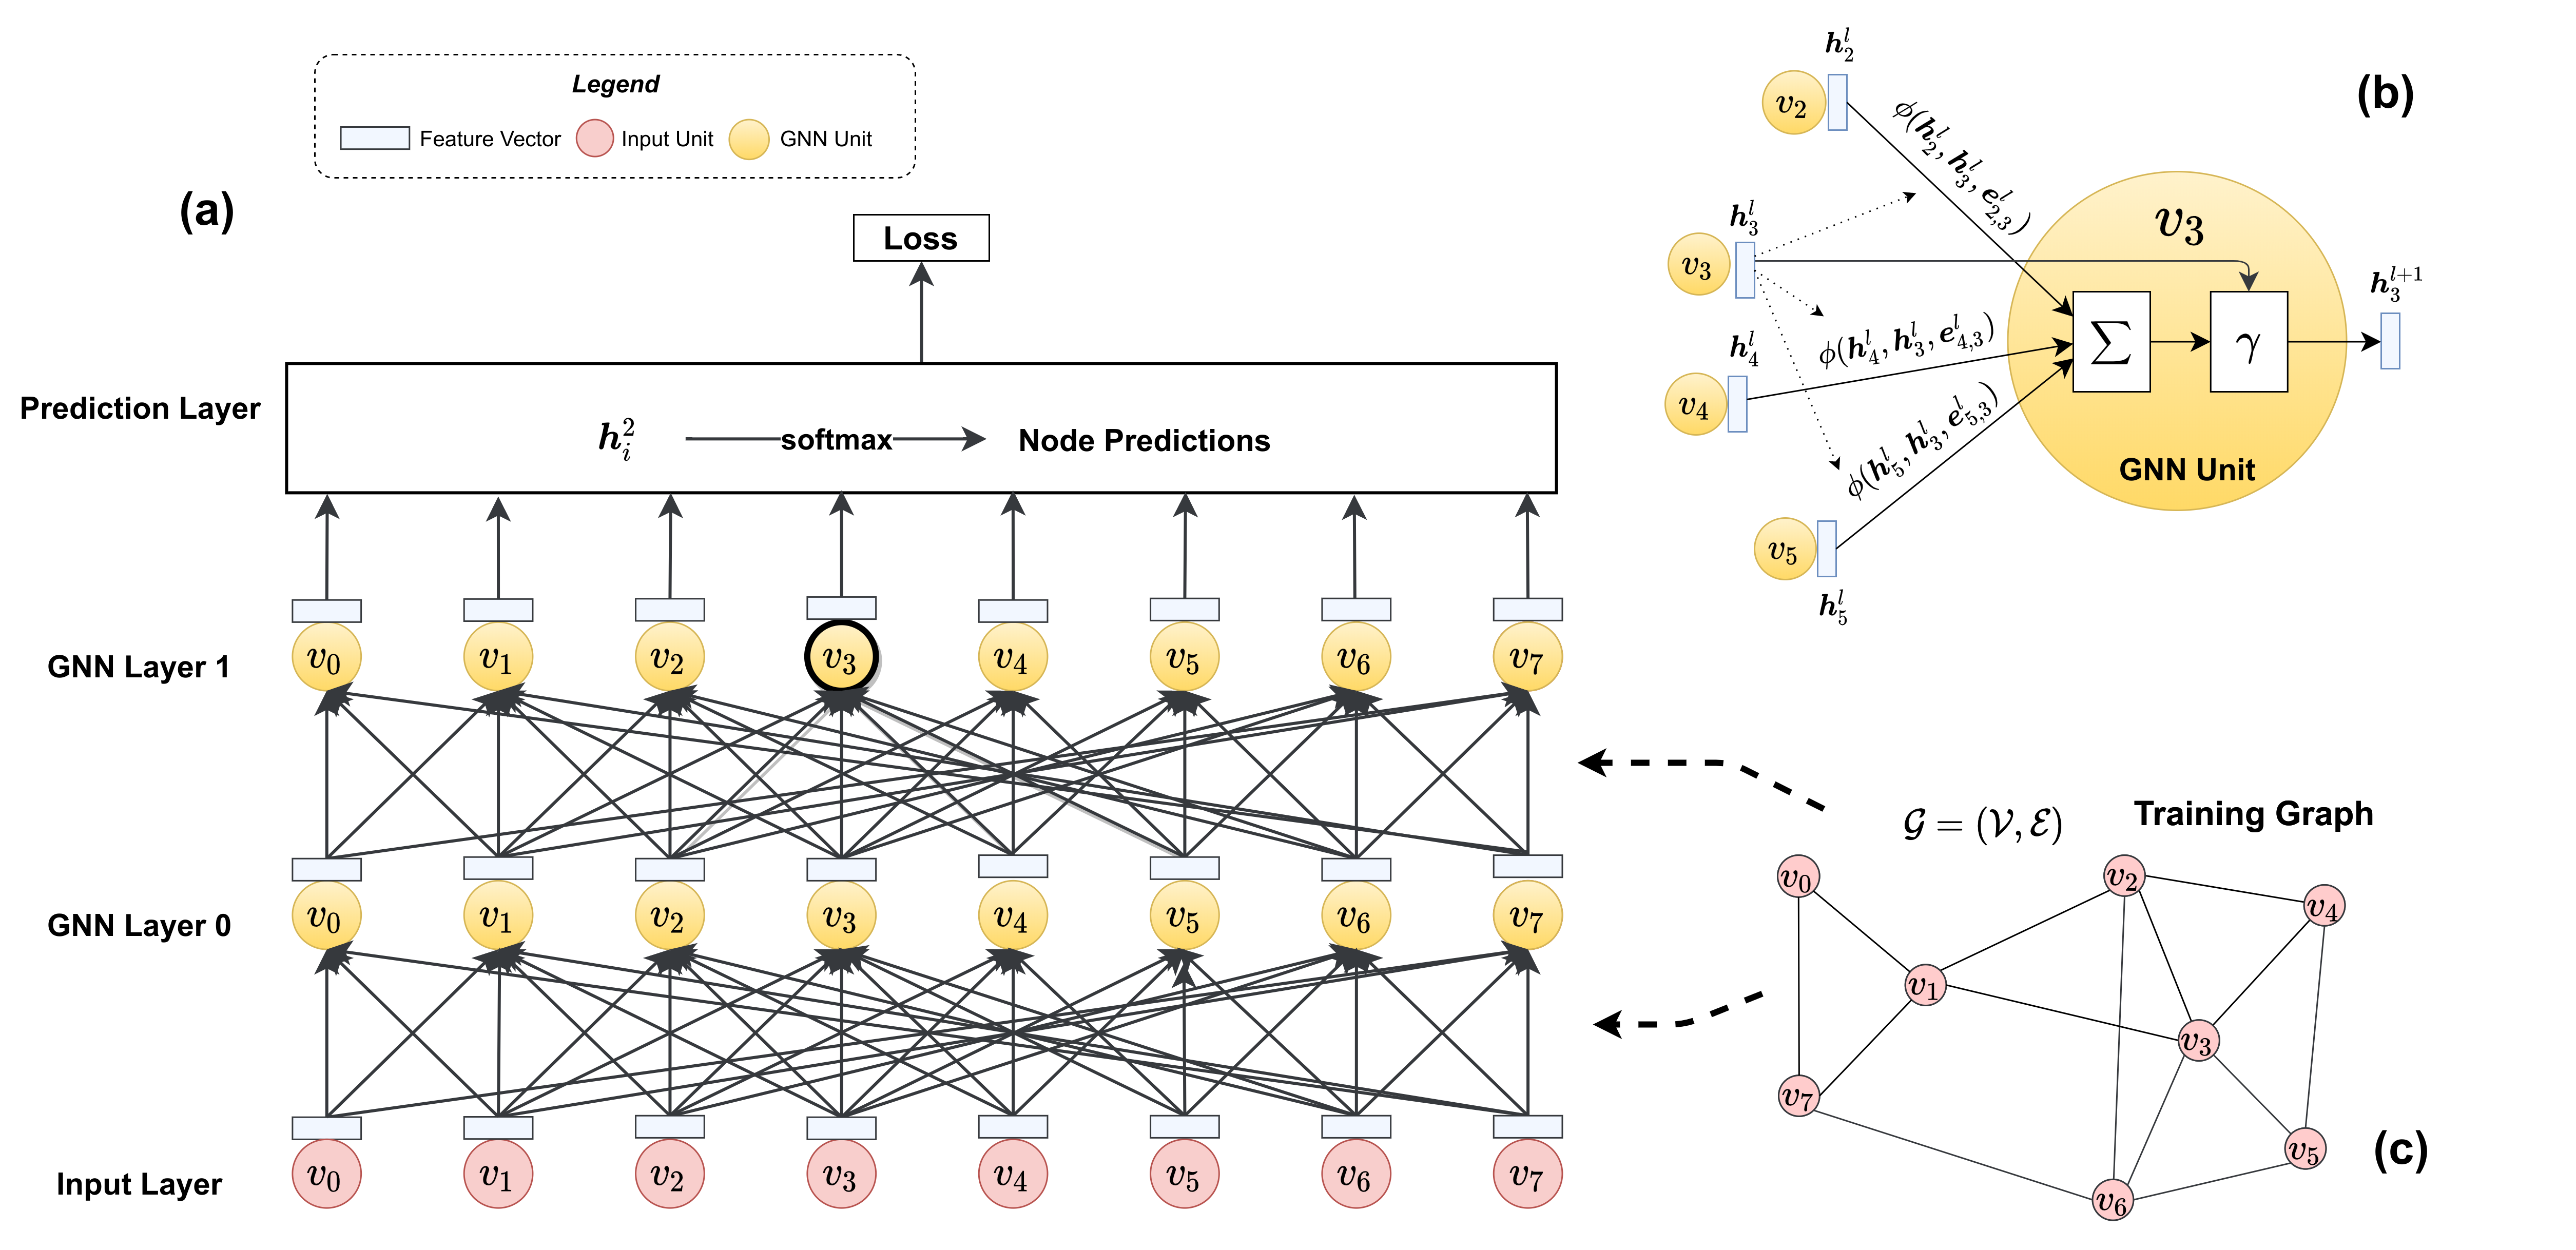
\includegraphics[width=0.95\columnwidth]{figs/illustration/GNN_common_architecture.png}
	\caption{Structure of a typical graph neural network. (a) Demo GNN; (b) GNN unit; (c) Demo graph. The target application is the node classification. The demo GNN has two GNN layers.}
	\label{fig:general_structure_of_gnn}
\end{figure}
